\subsection{Vectorization}
\label{sec:Vectorization}
Vectorization performed by Treebeard is enabled by the tiling transformations described in section \ref{sec:Tiling}. 
When the low level IR is translated to LLVM IR, Treebeard generates LLVM instructions that operate on the threholds and feature indices 
of nodes within a tile in a vector fashion. Therefore, thresholds and feature indices are loaded using vector loads and predicates are 
evaluated using vector comparisons. These vector LLVM IR instructions are then converted to vector instructions in the target ISA by 
the LLVM JIT.

The below listing shows some of the details of a vectorized tree walk. 
\begin{lstlisting}[style=c++]
  // A lookup table that determines the child index of
  // the next tile given the tile shape and the outcome
  // of the vector comparison on the current tile
  int16_t LUT[NUM_TILE_SHAPES, pow(2, TileSize)]
  
  ResultType Prediction_Function(...) {
    // ...
    Node n = getRoot(tree)
    while (isLeaf(tree, n)==false) do {
      thresholds = loadThresholds(tree, n)
      featureIndices = loadFeatureIndices(tree, n)
      // Gather required feature from the current row
      features = rows[i][featureIndices]
      // Vector comparison of features and thresholds
      comparison = features < thresholds
      
      // Pack bits in comparison vector into an integer
      comparisonIndex = combineBitsIntoInt(comparison)
      
      // Get child index of tile we need to move to
      tileShape = loadTileShape(tree, n)
      childIndex = LUT[tileShapeID, comparisonIndex]
      
      // Move to the correct child of the current node
      n = getChildNode(tree, n, childIndex) 
    }
    ThresholdType prediction = getLeafValue(n)
    // ...
  }  
\end{lstlisting}
To evaluate the current tile, the vector of thresholds is first loaded (\texttt{loadThresholds}). This vector contains the thresholds of all nodes in the tile. Then, the features required for comparison are gathered into a vector (lines 11 and 13). The feature vector is compared to the threshold vector and the child tile to move to is determined (lines 15 to 25). More details about tile shapes and the look up table are presented in subsequent sections.

\subsubsection{Tile Shapes}
Informally, the \textbf{\emph{tile shape}} is the shape of the region that encloses all nodes in a tile in a diagram of the decision tree. More formally, for a tile size $n_t$, each unique legal binary tree containing $n_t$ nodes (nodes being indistinguishable) corresponds to a tile shape.

Figure \ref{Fig:TileSize3Shapes} enumerates all tile shapes with a tile size of 3. There are a total of 5 tile shapes with size 3. The number of tile shapes with a tile size $n_t$, denoted by $NTS(n_t)$ is given by the following equation. 

\begin{equation}
  NTS(n) = \sum_{k=0}^{n-1} NTS(k) \times NTS(n-k-1)
\end{equation}

where $NTS(0) = NTS(1) = 1$.

\begin{figure}
  \centering
  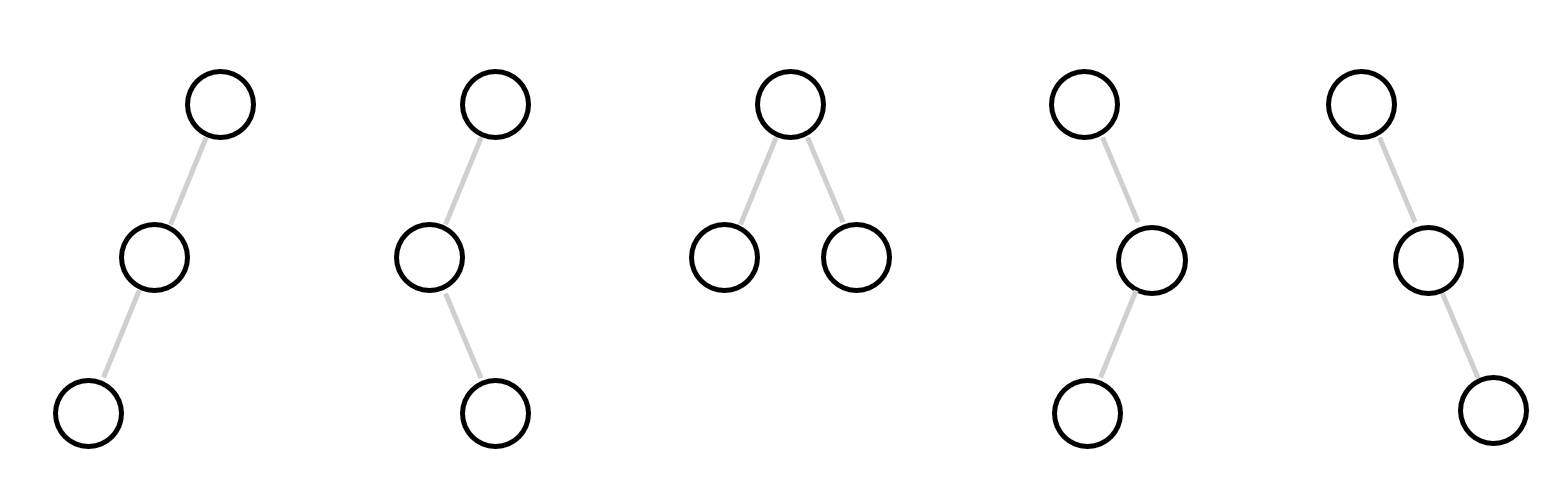
\includegraphics[width=\linewidth]{figures/TileShapes_Size3.PNG}
  \caption{All possible tile shapes with tile size $n_t=3$}
  \label{Fig:TileSize3Shapes}
\end{figure}

\subsubsection{Tile Shapes and Decision Tree Inference}
\label{Sec:TileShapesAndDecisionTreeInference}
Treebeard uses vector instructions to accelerate decision tree walks. Vector instructions are used to evaluate the predicates of all the nodes in a tile simultaneously. However, once the predicates of all the nodes in the tile are evaluated, computing the next tile to move to, given the outcome of the comparison depends on the tile shape of the current tile. To illustrate this problem, consider the case of the tiles of size 3 shown in figure \ref{Fig:TileTraversalTileSize3}. 
\begin{figure}
  \centering
  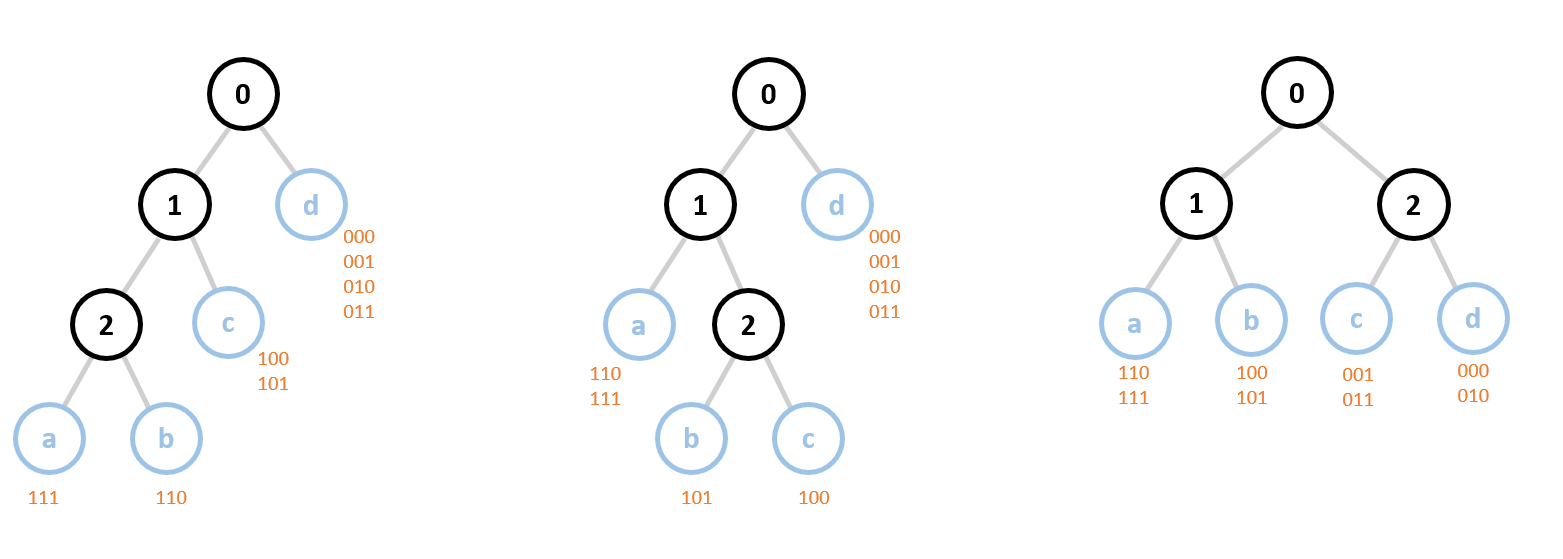
\includegraphics[width=\linewidth]{figures/TileTraversal_Size3.PNG}
  \caption{Example tile traversals with tile size $n_t=3$}
  \label{Fig:TileTraversalTileSize3}
\end{figure}
The diagram shows 3 of the 5 possible tile shapes for a tile size of 3. The nodes drawn in black are members of the tile $t_1$. The nodes in blue are the entry nodes of the children tiles of $t_1$. \TODO{Define entry nodes}

% To traverse a tile on an input row, first, the predicate of each node in the tile is computed. Subsequently, we need to determine which of the child tiles to move to next. Note that a true predicte (bit value 1) on a node implies a move to the left child and a false predicate (bit value 0) implies a move to the right child.

In the diagram, the bit strings (written in red) show which child we need to move to given the outcomes of the comparison. The bits represent the comparison outcomes of nodes and are in the order of the nodes in the tile -- marked 0, 1 and 2 in the diagram, i.e., the MSB is the predicate outcome of node 0 and the LSB the predicate outcome of node 2. For example, for the first tile shape, if the predicates of all nodes are true (i.e. the comparison outcome is 111), the next node to evaluate is $a$. 
% However, if the predicate of node 1 is false, then we need to move to $d$ regardless of the outcomes of nodes 2 and 3.
It is easy to see from the diagram that, depending on the tile shape, the same predicate outcomes can mean moving to different children. For example, for the outcome "011", the next tile is the 4th child (node $d$) for the first two tile shapes while it is the 3rd child for the other tile shape (node $c$).

\subsubsection{Lookup Table}
\label{sec:LookupTable}
A lookup table (LUT) is used to solve the problem described in section \ref{Sec:TileShapesAndDecisionTreeInference}, i.e. given the outcome of the comparisons of all nodes in a tile, determine the child tile we should evaluate next. The LUT is indexed by the tile shape and the comparison outcome. Formally, the LUT is a map.
\[
LUT : (TileShape, < Boolean \times n_t >) \rightarrow [0, n_t] \subset \mathbb{N}
\]

where $n_t$ is the tile size, $< Boolean \times n_t >$ is a vector of $n_t$ booleans. The value returned by the LUT is the index of the child of the current tile that should be evaluated next. For example, if we are evaluating the first tile $t$ in figure \ref{Fig:TileTraversalTileSize3}, and the result of the comparison is 110, then $LUT(TileShape(t), 110)=1$ since the tile we need to evaluate next is the tile with node $b$, which is the second child of the current tile.

In order to realize this LUT in generated code, Treebeard associates a non-negative integer ID with every unique tile shape of the given tile size. The result of the comparison, a vector of booleans, can be interpreted as a 64-bit integer. Therefore, the LUT can be implemented as a 2 dimensional array.
% \begin{lstlisting}{style=c++}
%   int16_t LUT[NTS(n_t), pow(2, n_t)]  
% \end{lstlisting}
Treebeard computes the values in the LUT statically as the tile size is a compile time constant.
\TODO{AP What comes after subsubsection?}

\subsection{In Memory Representation of Tiled Trees}
Treebeard currently has two in memory representations for tiled trees - an array based representation and a sparse representation. Both representations use an array of structs to represent all tiles of the model. 

\subsubsection{Array Based Representation}
\label{sec:ArrayBased}
Each tree in the model is represented as an array of tiles using the standard representation of trees as arrays. The root node is at index 0 and for a node at index $n$ in the array, the index of its $i^{th}$ child is given by $(n_t + 1) n + (i + 1)$ (nodes in the tree of tiles have $n_t + 1$ children). A tile is represented by an object of the following struct.
\begin{lstlisting}{style=c++}
  struct Tile {
    // A vector of TileSize elements
    <ThresholdType x TileSize> thresholds; 
    <FeatureIndexType x TileSize> featureIndices;
    // Integer that identifies the tile shape
    TileShapeIDType tileShapeID; 
  };  
\end{lstlisting}
\TODO{AP Is this level of detail really needed? Also, the vector type notation needs to be introduced somewhere.}
Even though this representation is simple and efficient for small models, the memory required for bigger models is very large. 
%The memory footprint is up to 20X that of the scalar representation.
This memory bloat causes performance problems because the span of the L1 TLB is not sufficient to efficiently translate 
addresses for the whole model. Storing leaves as full tiles (even though leaves just have to represent one value) and the
empty space introduced due to the array based representation of trees that are not complete account for most
of the increase.
%The sparse representation described next tries to address these issues. 

\subsubsection{Sparse Representation}
\label{sec:SparseRep}
The sparse representation tries to address the large memory footprint of the array based representation by doing the following.

\begin{itemize}
  \item We add a child pointer to each tile to eliminate the wasted space in the array representation. This points to the first child of the tile. All children of a tile are stored contiguously.
  \item Leaves are stored as a separate array of scalar values. Across all our benchmarks, after tiling a large fraction of 
  leaves are such that all their siblings are also leaves. Such leaves are directly moved into the leaves array. For leaves
  for which this property does not hold, an extra ``hop'' is added by making the original leaf tile a normal tile. All its
  children are made leaves with the same value as the original leaf.
\end{itemize}

\begin{figure}
  \centering
  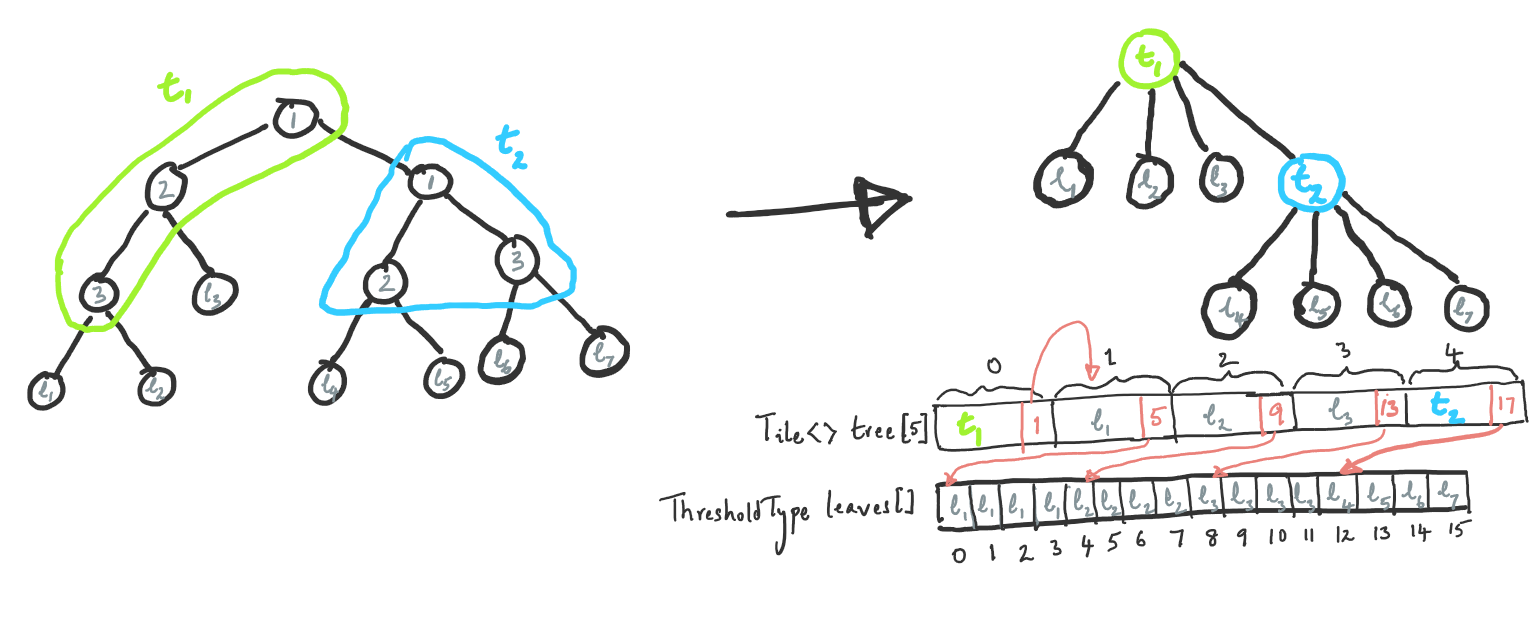
\includegraphics[width=\linewidth]{figures/SparseRep_TileSize3.PNG}
  \caption{Sparse representation with tile size $n_t=3$}
  \label{Fig:SparseRep}
\end{figure}

Figure \ref{Fig:SparseRep} shows some of the details of the sparse representation.
% The tree on the left of the diagram is the actual decision tree with the nodes grouped into tiles $t_1$ and $t_2$. The tree on the right is the tree of tiles.
The arrays depicted below show how the tree is represented in memory. The first array ($\texttt{tree}$) is an array of tiles 
and has 5 elements. Each element of the array represents a single tile and has the thresholds of the nodes, the feature
indices, a tile shape ID and a pointer to the first child (shown explicitly in red). 

As a specific example, consider the tile $t_1$. The tile has four children -- $l_1$, $l_2$, $l_3$ and $t_2$ in that order (left to right). These tiles are stored contiguously in the $\texttt{tree}$ array and a pointer to the first of these, $l_1$ is stored in the tile $t_1$ (the index 1 is stored in the tile $t_1$ as shown). 

Now consider the tile $t_2$. Since all children of the tile $t_2$ are leaves, they are all moved into the $\texttt{leaves}$ array.
To store a pointer into the $\texttt{leaves}$ array, we add $\texttt{len(tree)}$ to the element index in the $\texttt{leaves}$ array.
The tile $t_2$'s child is the element at index 12 of the $\texttt{leaves}$ array. Therefore, the index $12 + 5 = 17$ is stored in 
the tile $t_2$. Any index $i$ that is greater than the length of the $\texttt{tree}$ array is regarded as an index into the
$\texttt{leaves}$ array. The index into the $\texttt{leaves}$ array is $i - \texttt{len(tree)}$.

The other aspect of the representation is that an extra hop is added for the leaves $l_1$, $l_2$ and $l_3$ in order to simplify
code generation. This enforces the invariant that all leaves are stored in the leaves array and  simplifies checking whether
we've reached a leaf. Therefore, 4 new leaves are added as children for each of the original leaves $l_1$, $l_2$ and $l_3$. 
Each of these 12 newly added leaves has the same value as its parent. These are the first 12 elements of the $\texttt{leaves}$ array.

Even though we currently have implementations of the two representations detailed in sections \ref{sec:ArrayBased} 
and \ref{sec:SparseRep}, support for other representations is not hard to add. All optimizing passes that work on 
the high level and mid level IR will continue to work as is. Programmers need only provide new lowering passes for
a few operations in the low level IR.

\subsubsection{Code Generation for Probability Based Tiling}
As probability based tiling pulls the most probable leaves of a decision tree nearest the root, it poses 
some implementation challenges. By design, the tiling process makes the tree of tiles 
imbalanced. The array based representation (section \ref{sec:ArrayBased})
cannot be used because of the memory footprint increase (a large part of the tree is empty, but would need to be allocated).
On the other hand, the sparse representation in section \ref{sec:SparseRep} adds 
an extra hop for leaves that have non-leaf siblings. But this would mean that we add extra hops for 
the most probable leaves after probability based tiling which defeats the optimization.
\TODO{kr: connect to Peeling in MIR}
We address these challenges using a code generation strategy. Treebeard peels 
the tree walk and specializes the leaf checks at higher levels to avoid the extra hop. Currently, 
we determine the maximum depth of leaves needed to cover 90 percent of the inputs and peel the tree 
walk by as many iterations. For example, consider the case where leaves until depth 2 are needed to 
cover 90 percent of the training input. Then, Treebeard generates the following IR. 

\begin{lstlisting}{style=c++}
    // ...
    tree = getTree(forest, t)
    node = getRoot(tree)
    node = traverseTreeTile(tree, node, rows[i])
    if (isLeafTile(node)) {
        treePrediction = getLeafValue(tree, node)
    } else {    
        node = traverseTreeTile(tree, node, rows[i])
        if (isLeafTile(node)) {
            treePrediction = getLeafValue(tree, node)
        } else {    
            // Loop based traversal 
        }
    }
    treePrediction = getLeafValue(tree, node)
    // ...
\end{lstlisting}

The if statements check whether a node is a leaf tile and hence avoid the extra hop. 
%The memory 
%requirement is also not increased because only a small fraction of leaves are represented as full tiles.
While walk peeling is used to improve the performance of probability based tiling by specializing leaf tests,
the transformation is by itself general and can be used in different contexts. For example, it could be used 
to elide leaf checks until a depth $d$ is reached if we know all leaves are at a depth greater than $d$. 

One other issue that the code generator needs to handle is that walks of different trees in the same ensemble may 
need to be peeled to different depths. A strategy similar to what is used for uniform tiling is used to handle this.
Trees are reordered so that all trees 
with equal peeling depth are grouped together and the loops in the IR are fissed so that tree walks 
for these groups of trees can be specialized differently.
% This is very similar to the code generation strategy used for uniform tiling.
